\clearpage
\item \subquestionpoints{5} \textbf{Coding problem.}
Follow the instructions in \texttt{src/p01b\_logreg.py} to train a
logistic regression classifier using Newton's Method.
Starting with $\theta = \vec{0}$, run Newton's Method until the updates to
$\theta$ are small: Specifically,  train until the first iteration $k$ such
that $\|\theta_{k} - \theta_{k-1}\|_1 < \epsilon$, where
$\epsilon = 1\times 10^{-5}$. Make sure to write your model's predictions to
the file specified in the code.

\ifnum\solutions=1 {
  \begin{answer}
\begin{figure}[h]
  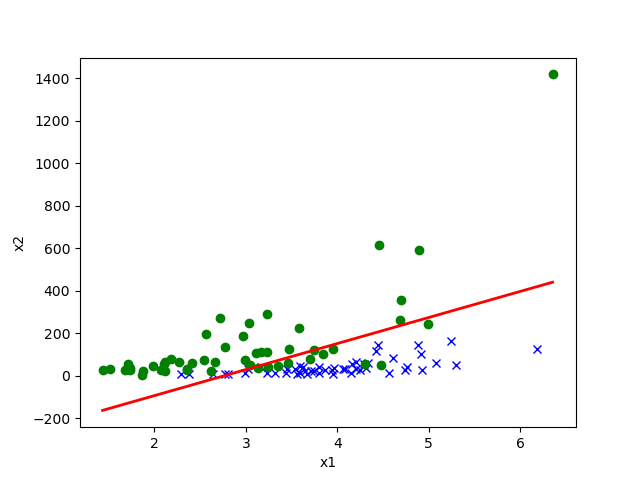
\includegraphics[height=5.5cm]{C:/Users/feroc/OneDrive/Notability/CS229 Machine Learning/problem_sets/ps1/src/output/p01b_pred_1.png}
  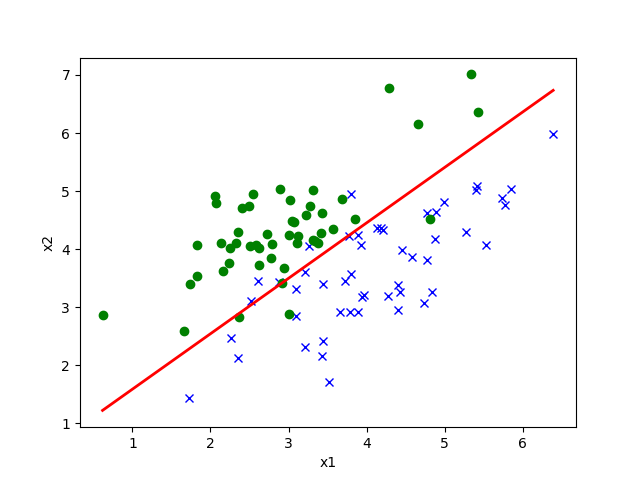
\includegraphics[height=5.5cm]{C:/Users/feroc/OneDrive/Notability/CS229 Machine Learning/problem_sets/ps1/src/output/p01b_pred_2.png}
\end{figure}
\end{answer}

} \fi
